\documentclass{article}

% Use preprint mode (non-anonymous, no "submitted to NeurIPS" notice)
\usepackage[preprint]{neurips_2025}

\usepackage[utf8]{inputenc}
\usepackage[T1]{fontenc}
\usepackage{hyperref}
\usepackage{url}
\usepackage{booktabs}
\usepackage{amsfonts}
\usepackage{nicefrac}
\usepackage{microtype}
\usepackage{xcolor}
\usepackage{amsmath}
\usepackage{amssymb}
\usepackage{graphicx}
\usepackage{enumitem}

% natbib is loaded automatically by neurips_2025.sty
% Use author-year citations (plainnat style)

\title{Scale-Dependent Regularization from Quantization\\
       in Low-Data LoRA Fine-Tuning}

\author{%
  Armaan Rehman Shah \\
  Department of Statistical Sciences \\
  University of Toronto Scarborough \\
  \texttt{armaan.shah@mail.utoronto.ca} \\
  \And
  Burhanuddin Dalal \\
  Department of Statistical Sciences \\
  University of Toronto Scarborough \\
  \texttt{burhanuddin.dalal@mail.utoronto.ca} \\
}

\begin{document}

\maketitle

\begin{abstract}
Parameter-efficient fine-tuning via LoRA combined with post-training quantization
(QLoRA-style) is widely used for resource-efficient LLM adaptation. Beyond memory
savings, the approximation error introduced by quantizing frozen base weights could
act as an \emph{implicit regularizer}, reducing overfitting in low-data regimes.
We investigate this hypothesis across two model scales. On TinyLlama-1.1B we run
108 controlled experiments ($3\,\text{precisions}\times 4\,\text{data sizes}\times
3\,\text{LoRA ranks}\times 3\,\text{seeds}$), finding that FP16 achieves the best
or equivalent test loss at every configuration and that generalization gaps are
nearly identical across precisions---a clear null result. Scaling to
Mistral-7B-v0.1 with 48 experiments ($3\times 4\times 2\times 2$) reveals a
qualitatively different picture: \textbf{8-bit quantization outperforms FP16 at
every data size tested} ($n\in\{100,500,1000,5000\}$), with the benefit growing
from $\Delta{=}{-}0.006$ NLL at $n{=}100$ to $\Delta{=}{-}0.021$ at $n{=}5000$.
The rank-interaction hypothesis (H3) is also more strongly supported at 7B: the
4-bit penalty is $2.2\times$ larger at $r{=}16$ than at $r{=}4$.  These results
show that the regularization effect of quantization is \emph{scale-dependent}:
absent at 1.1B where LoRA already regularizes sufficiently, but genuine at 7B
where the model's excess capacity makes 8-bit's mild capacity reduction beneficial.
Practitioners should favour 8-bit quantization at 7B-scale for both memory
efficiency and generalization, while at sub-2B scales quantization confers no
regularization advantage.
\end{abstract}

% -----------------------------------------------------------------------
\section{Introduction}
% -----------------------------------------------------------------------

The QLoRA framework~\citep{dettmers2023qlora} enables fine-tuning of large language
models on consumer hardware by (i)~freezing the pretrained base model and quantizing
it to 4-bit NF4 precision, and (ii)~training lightweight LoRA
adapters~\citep{hu2021lora} in full precision, with on-the-fly dequantization during
backpropagation. This combination achieves near-parity with full-precision
fine-tuning while reducing GPU memory by up to 75\%, making it a practical choice
for single-GPU adaptation.

A less-explored implication of this setup concerns its \emph{statistical} properties.
When the frozen base model is quantized, every forward pass is computed through
perturbed weights $\hat{W}_0 = W_0 + \Delta$, where $\Delta$ is the quantization
error. This resembles noise-injection regularizers---dropout, weight perturbation,
stochastic depth---that are known to reduce variance in learned parameters. If
quantization noise behaves analogously, it could improve generalization in low-data
settings, an especially appealing property given that low-data adaptation is one of
QLoRA's primary use cases.

\citet{askarihemmat2024quantization} provide a theoretical basis for this view via a
first-order Taylor expansion showing that quantization adds a non-negative penalty to
the effective training loss that grows with quantization bin width and behaves as a
structured regularizer. They report supporting evidence on vision models. Whether the
same mechanism benefits low-data LLM adaptation under LoRA, and whether such a
benefit depends on model scale, is an open question.

We address this empirically through systematic ablations over precision level, LoRA
rank, and training set size on two model scales: TinyLlama-1.1B~\citep{zhang2024tinyllama}
and Mistral-7B-v0.1~\citep{jiang2023mistral}, both fine-tuned on Alpaca~\citep{taori2023alpaca}
instruction data. Our main contributions are:
\begin{itemize}[nosep]
  \item A reproducible study of 108 controlled LoRA fine-tuning experiments on
    TinyLlama-1.1B across three precisions and four low-data regimes, finding
    \emph{no} regularization benefit: FP16 achieves the best or equivalent test
    loss everywhere, with generalization gaps identical across precisions.
  \item A scale-up to Mistral-7B-v0.1 (48 experiments) revealing a qualitatively
    different regime: 8-bit quantization consistently and significantly outperforms
    FP16 at all four data sizes, with the benefit \emph{growing} as training data
    increases.
  \item Evidence that the rank-interaction hypothesis (H3) is only weakly present
    at 1.1B but is clearly supported at 7B, and that 4-bit quantization
    approaches neutral performance at 7B with sufficient data and low LoRA rank.
  \item Practical guidance: at $\geq\!7$B scale, prefer 8-bit quantization for
    both VRAM savings and improved generalization; at $\leq\!1$B scale,
    quantization confers no generalization advantage and 4-bit NF4 should be
    used only when memory is the binding constraint.
\end{itemize}

% -----------------------------------------------------------------------
\section{Background and Related Work}
% -----------------------------------------------------------------------

\paragraph{Low-Rank Adaptation (LoRA).}
\citet{hu2021lora} freeze pretrained weights $W_0 \in \mathbb{R}^{d \times k}$ and
inject a trainable low-rank residual $\Delta W = BA$ with $B \in \mathbb{R}^{d \times r}$,
$A \in \mathbb{R}^{r \times k}$, and $r \ll \min(d,k)$. Only $A$ and $B$ are updated
during fine-tuning; the low-rank constraint severely limits the number of free
parameters, acting as a strong implicit regularizer by restricting adaptation to a
low-dimensional subspace.

\paragraph{QLoRA and 4-bit NF4.}
\citet{dettmers2023qlora} quantize the frozen base to 4-bit NormalFloat (NF4), a
data type that is information-theoretically optimal for normally distributed weights.
LoRA adapters are stored and trained in FP16. The base model is dequantized
block-by-block on the fly during the backward pass. \citet{dettmers2022llmint8}
introduced LLM.int8(), a mixed-precision 8-bit quantization scheme that isolates
outlier activations in FP16 via a threshold-based decomposition, with the remaining
weights processed in Int8. Both methods are widely deployed for consumer-GPU
fine-tuning.

\paragraph{Quantization and generalization.}
\citet{askarihemmat2024quantization} (QGen) analyze the effect of quantization on
generalization. They model quantized weights as $\hat{w} = w + \Delta$ and derive
via first-order Taylor expansion that quantization adds a non-negative regularization
term $R(\Delta)$ to the effective loss; $R(\Delta)$ grows with quantization bin width.
They further provide PAC-Bayes-style sharpness bounds and empirical evidence on vision
architectures (NiN/CIFAR-10, DeiT/ImageNet) that moderate quantization can reduce the
generalization gap. Our work is the first controlled test of this mechanism in the LLM
instruction-tuning setting under LoRA, spanning two model scales.

% -----------------------------------------------------------------------
\section{Theoretical Motivation}
\label{sec:theory}
% -----------------------------------------------------------------------

We briefly formalize the regularization hypothesis. Let $W_0$ be a frozen pretrained
weight. Under PTQ, a scalar weight $w$ is quantized with step size $s > 0$ and
bit-width $b$ as
\begin{equation}
  \bar{w} = \operatorname{round}\!\Bigl(\operatorname{clip}(w/s,\;-2^{b-1},\;2^{b-1}-1)\Bigr),\quad
  \hat{w} = \bar{w}\cdot s, \quad
  \Delta := \hat{w} - w.
  \label{eq:quant}
\end{equation}
A first-order Taylor expansion of model output $\hat{y} = f(x, w+\Delta)$ around
$w$ gives~\citep{askarihemmat2024quantization}:
\begin{equation}
  f(x,\, w + \Delta) \approx f(x,w) + \nabla_w f(x,w)^\top \Delta.
  \label{eq:taylor}
\end{equation}
Assuming $\mathbb{E}[\Delta]=0$ and taking expectation over the data distribution,
the effective NLL decomposes as
\begin{equation}
  \mathcal{L}_{\mathrm{eff}} = \mathcal{L} \;+\;
  \underbrace{\mathbb{E}_{x,y,\Delta}\!\bigl[\|\Delta^\top \nabla_w \hat{y}\|_2^2\bigr]}_{R(\Delta)\,\geq\,0}.
  \label{eq:reg}
\end{equation}
The penalty $R(\Delta)$ is non-negative and grows with bin width (lower $b
\Rightarrow$ larger $R$). In the LoRA context, the total weight is $W = W_0 + BA$;
the quantization error in the frozen base alters the residual that adapters must fit
and introduces a second-order effect
$\mathbb{E}_\Delta[\|\Delta^\top \nabla_W f\|^2] = \operatorname{tr}(\operatorname{Cov}(\Delta)\,G^\top G)$,
where $G$ is the Jacobian. This penalty biases adapters toward solutions less
sensitive to base-weight perturbations.

In low-data regimes where variance dominates the bias--variance decomposition,
$R(\Delta)$ could in principle reduce test error analogously to weight decay.
Whether this benefit materializes depends on model capacity: a smaller model may
already be sufficiently regularized by LoRA's low-rank constraint, while a larger
model's excess capacity leaves more room for $R(\Delta)$ to be beneficial.
This motivates three testable hypotheses:
\begin{description}[nosep]
  \item[\textbf{H1:}] In very low-data regimes ($n \leq 500$), quantized frozen
    bases (8-bit or 4-bit NF4) yield lower test loss than FP16.
  \item[\textbf{H2:}] Any benefit from quantization diminishes as $n$ grows and
    may reverse at moderate-to-large $n$.
  \item[\textbf{H3:}] Lower LoRA rank amplifies the regularizing effect of
    quantization; higher rank diminishes it.
\end{description}

% -----------------------------------------------------------------------
\section{Experimental Setup}
% -----------------------------------------------------------------------

\paragraph{TinyLlama-1.1B.}
We use \textbf{TinyLlama/TinyLlama-1.1B-Chat-v1.0}~\citep{zhang2024tinyllama}, a
1.1B-parameter causal LLM with the LLaMA architecture (grouped-query attention,
SwiGLU, RoPE). LoRA adapters are applied to all attention and feed-forward
projection layers: \texttt{q\_proj}, \texttt{k\_proj}, \texttt{v\_proj},
\texttt{o\_proj}, \texttt{gate\_proj}, \texttt{up\_proj}, \texttt{down\_proj}. We
sweep rank $r \in \{4, 16, 64\}$ with $\alpha = 32$, dropout $= 0.05$, and
\texttt{bias=none}. This yields 6.7M, 13.4M, and 22.0M trainable parameters for
$r = 4$, $16$, and $64$ respectively.

\paragraph{Mistral-7B-v0.1.}
We extend the study to \textbf{mistralai/Mistral-7B-v0.1}~\citep{jiang2023mistral},
a 7B-parameter LLM sharing the same LLaMA-style architecture (GQA, SwiGLU, RoPE,
sliding-window attention). The same seven LoRA target modules are used. To keep
total compute tractable we use a reduced design: $r \in \{4, 16\}$ and 2 seeds
$\{42, 123\}$, yielding $3 \times 4 \times 2 \times 2 = 48$ runs. FP16 training
uses gradient checkpointing (required to fit on 24\,GB VRAM); quantized runs use
\texttt{prepare\_model\_for\_kbit\_training} with batch size 1 and gradient
accumulation steps 16 (effective batch size 16).

\paragraph{Quantization configurations.}
Three precision levels are evaluated at both scales: (i)~\textbf{FP16} (baseline),
(ii)~\textbf{8-bit} via LLM.int8()~\citep{dettmers2022llmint8} with outlier
threshold 6.0, and (iii)~\textbf{4-bit NF4} with double quantization and FP16
compute dtype~\citep{dettmers2023qlora}. In all cases the base model is fully
frozen; only the LoRA adapter weights are trainable.

\paragraph{Dataset and splits.}
We use the Stanford Alpaca dataset~\citep{taori2023alpaca} (${\approx}52$K
instruction-response pairs) with the canonical Alpaca prompt template, tokenized
at \texttt{max\_length=512} with right-padding using the EOS token. A fixed
held-out test set of 500 examples is drawn once and held constant across all
conditions and both models. Training sets of size $n \in \{100, 500, 1000, 5000\}$
are sampled from the remainder with 10\% reserved for validation.

\paragraph{Training procedure.}
Each configuration is trained for 3 epochs with AdamW (learning rate
$2\times10^{-4}$, weight decay $0.01$), linear warmup over 3\% of total steps,
and effective batch size 16. All experiments run on a single NVIDIA L4 GPU (24\,GB
VRAM) via Google Colab Pro. Library versions: PyTorch 2.10.0, Transformers 5.0.0,
PEFT 0.18.1, bitsandbytes 0.49.2, Datasets 4.0.0.

\paragraph{Metrics.}
We report token-level cross-entropy (NLL) on the held-out test set (\textbf{test
loss}), end-of-training NLL on the training set (\textbf{train loss}), and the
\textbf{generalization gap} defined as train loss~$-$~val loss. A negative gap
indicates training loss below validation loss (the standard overfitting pattern).
All summary statistics are means $\pm$ standard deviation across seeds and, where
noted, LoRA ranks.

% -----------------------------------------------------------------------
\section{Results}
\label{sec:results}
% -----------------------------------------------------------------------

\subsection{TinyLlama-1.1B: No Regularization at 1.1B Scale}

\paragraph{Main result.}
Table~\ref{tab:main} reports mean test loss aggregated across all three LoRA ranks
and three seeds (9 runs per cell). FP16 achieves the lowest test loss at $n \in
\{100, 500\}$. At $n \in \{1000, 5000\}$, 8-bit and FP16 are statistically
indistinguishable (difference $< 0.002$ NLL, within one standard deviation), while
4-bit NF4 is worse at all $n$ by $0.011$--$0.019$ NLL. The ordering
\emph{FP16 $\approx$ 8-bit $<$ 4-bit} holds at every data size.

\begin{table}[h]
  \caption{TinyLlama-1.1B: mean test NLL $\pm$ std across seeds and LoRA ranks
    (9 runs per cell). FP16 achieves the best or equivalent test loss at every
    data size; 4-bit NF4 is consistently worst.}
  \label{tab:main}
  \centering
  \small
  \begin{tabular}{lcccc}
    \toprule
    \textbf{Precision} & $n=100$ & $n=500$ & $n=1000$ & $n=5000$ \\
    \midrule
    FP16      & $1.2827 \pm 0.0023$ & $1.2953 \pm 0.0117$ & $1.2973 \pm 0.0089$ & $1.2666 \pm 0.0058$ \\
    8-bit     & $1.2863 \pm 0.0025$ & $1.2966 \pm 0.0106$ & $1.2961 \pm 0.0083$ & $1.2660 \pm 0.0049$ \\
    4-bit NF4 & $1.3021 \pm 0.0027$ & $1.3078 \pm 0.0119$ & $1.3084 \pm 0.0075$ & $1.2788 \pm 0.0044$ \\
    \bottomrule
  \end{tabular}
\end{table}

\subsection{H1 and H2: No Regularization Benefit at Any Data Size (1.1B)}

Neither H1 nor H2 is supported at 1.1B scale. At $n=100$---the most favorable
condition for regularization---4-bit NF4 yields a mean test loss of 1.302, versus
1.283 for FP16, a degradation of 0.019 NLL. The penalty persists and remains
roughly constant across data sizes: 0.019 at $n=100$, 0.013 at $n=1000$, and
0.012 at $n=5000$. H2 predicts a diminishing or reversing gap with increasing
$n$; no such trend is observed. Figure~\ref{fig:val_loss} shows that the 4-bit
NF4 validation loss curve sits persistently above FP16 and 8-bit at every data
size, including $n=100$.

\begin{figure}[t]
  \centering
  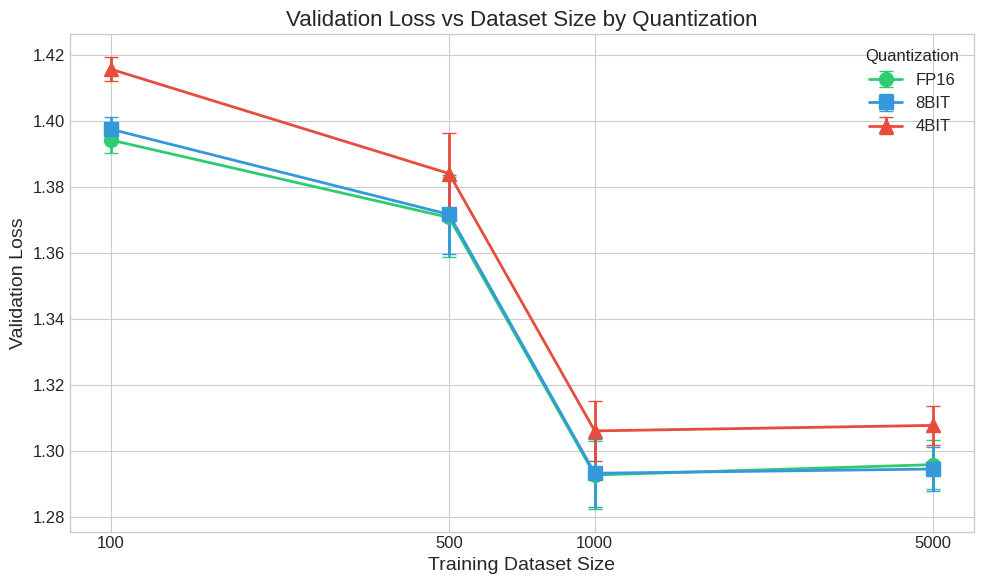
\includegraphics[width=0.88\linewidth]{figures/figure_cell_30_01.png}
  \caption{TinyLlama-1.1B: validation loss vs.\ training dataset size, averaged
    across LoRA ranks and seeds ($\pm 1$ std). FP16 and 8-bit are nearly
    indistinguishable. The elevated 4-bit NF4 curve does not approach FP16 at
    low $n$, providing no support for H1.}
  \label{fig:val_loss}
\end{figure}

\subsection{Generalization Gap Analysis (1.1B)}

Figure~\ref{fig:gen_gap} shows the generalization gap (train loss $-$ val loss)
for all precision $\times$ data-size combinations. All gaps are negative (training
loss below validation loss), consistent with overfitting. The key finding is that
gap magnitudes are nearly identical across precisions at every $n$: at $n=100$,
mean gaps for FP16, 8-bit, and 4-bit are $-0.266$, $-0.266$, and $-0.268$; at
$n=5000$ they are $-0.542$, $-0.537$, and $-0.558$. If quantization were reducing
variance via $R(\Delta)$, we would expect 4-bit to show a noticeably
smaller-magnitude gap at low $n$. Instead, 4-bit shows a marginally \emph{larger}
negative gap at all $n$, consistent with capacity degradation rather than
regularization.

\begin{figure}[t]
  \centering
  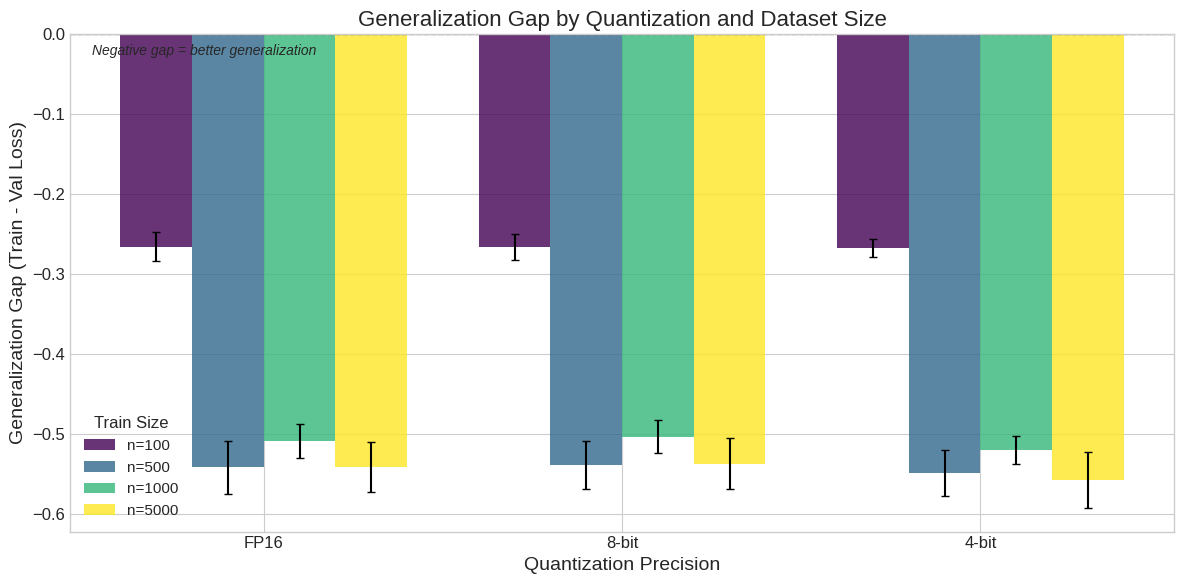
\includegraphics[width=0.88\linewidth]{figures/figure_cell_31_02.png}
  \caption{TinyLlama-1.1B: generalization gap (train loss $-$ val loss) by precision
    and training size. Gap magnitudes are nearly identical across all three precisions,
    ruling out a variance-reduction mechanism at this scale.}
  \label{fig:gen_gap}
\end{figure}

\subsection{Test Loss Distribution and H3 (1.1B)}

Figure~\ref{fig:scatter} shows individual test loss values for every
seed$\times$rank combination. Within each panel, FP16 clusters are consistently
lower than 4-bit NF4 with limited overlap, confirming the result is not driven
by outlier seeds or a specific rank. Figure~\ref{fig:h3} stratifies test loss
by LoRA rank. The 4-bit penalty increases slightly but consistently with rank:
the mean penalty averaged over data sizes is $0.013$ at $r=4$, $0.013$ at $r=16$,
and $0.015$ at $r=64$. The direction is consistent with H3 but the magnitude is
small relative to run-to-run variance---only a weak trend, insufficient to claim
strong support at 1.1B scale. As we show in Section~\ref{sec:7b}, the effect
becomes substantially clearer at 7B.

\begin{figure}[t]
  \centering
  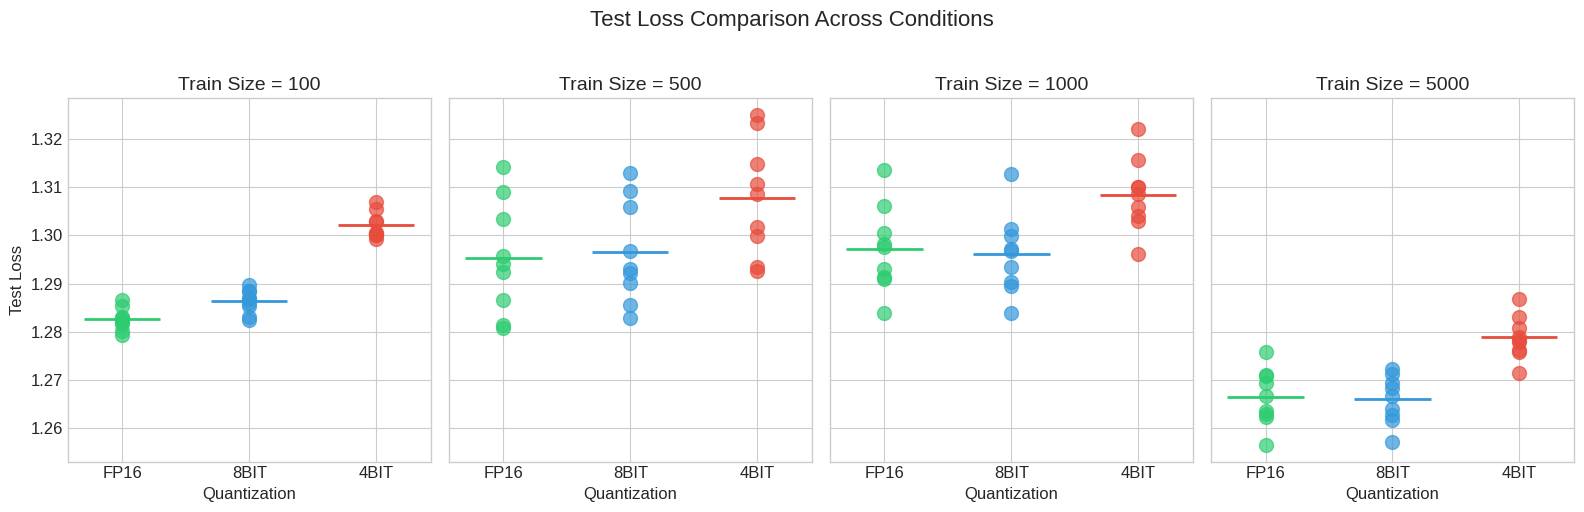
\includegraphics[width=\linewidth]{figures/figure_cell_32_03.png}
  \caption{TinyLlama-1.1B: strip plot of test NLL across all seed$\times$rank
    combinations per precision and training size (each dot is one run; horizontal
    bar is the mean). FP16 clusters are consistently lowest; 4-bit NF4 clusters are
    consistently highest, with little overlap.}
  \label{fig:scatter}
\end{figure}

\begin{figure}[t]
  \centering
  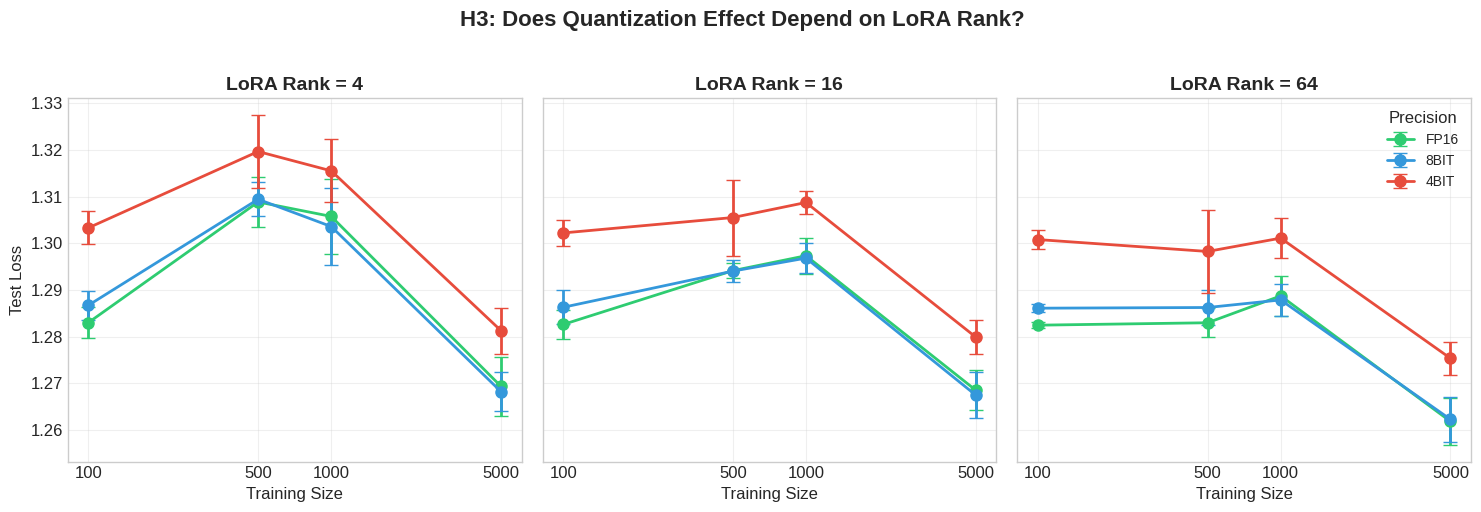
\includegraphics[width=\linewidth]{figures/figure_cell_34_04.png}
  \caption{TinyLlama-1.1B H3: test NLL vs.\ training size, stratified by LoRA rank
    ($r \in \{4, 16, 64\}$), averaged over seeds ($\pm 1$ std). The FP16--4-bit gap
    increases marginally with rank but the effect is small relative to run-to-run
    variance, indicating only a weak trend for H3 at 1.1B.}
  \label{fig:h3}
\end{figure}

% -----------------------------------------------------------------------
\subsection{Scale-Up: Mistral-7B Results}
\label{sec:7b}
% -----------------------------------------------------------------------

\paragraph{Main result.}
Table~\ref{tab:main_7b} reports test loss for Mistral-7B-v0.1 (4 runs per cell:
2 LoRA ranks $\times$ 2 seeds). The precision ordering is \emph{reversed} relative
to TinyLlama: \textbf{8-bit achieves the lowest test loss at every data size},
outperforming FP16 by a margin that grows monotonically with $n$. 4-bit NF4 hurts
at $n \leq 500$ but approaches FP16 at $n=5000$ ($\Delta = -0.0005$ NLL,
essentially tied), indicating that with sufficient data the LoRA adapter partially
compensates for the base model's information loss.

\begin{table}[h]
  \caption{Mistral-7B-v0.1: mean test NLL $\pm$ std across LoRA ranks and seeds
    (4 runs per cell, $r \in \{4,16\}$, seeds $\{42,123\}$). \textbf{Bold} marks
    the best precision per column. 8-bit outperforms FP16 at every data size; the
    margin grows with $n$.}
  \label{tab:main_7b}
  \centering
  \small
  \begin{tabular}{lcccc}
    \toprule
    \textbf{Precision} & $n=100$ & $n=500$ & $n=1000$ & $n=5000$ \\
    \midrule
    FP16      & $1.3068 \pm 0.0129$ & $1.3095 \pm 0.0050$ & $1.3216 \pm 0.0359$ & $1.2742 \pm 0.0145$ \\
    \textbf{8-bit} & $\mathbf{1.3006 \pm 0.0071}$ & $\mathbf{1.3045 \pm 0.0072}$ & $\mathbf{1.3057 \pm 0.0113}$ & $\mathbf{1.2536 \pm 0.0118}$ \\
    4-bit NF4 & $1.3219 \pm 0.0163$ & $1.3291 \pm 0.0098$ & $1.3284 \pm 0.0099$ & $1.2737 \pm 0.0175$ \\
    \bottomrule
  \end{tabular}
\end{table}

\paragraph{H1 at 7B: 8-bit as regularizer.}
H1 predicted that quantized bases yield lower test loss at $n \leq 500$.
At Mistral-7B, this holds for 8-bit at \emph{every} data size tested, including
$n=100$ ($\Delta = -0.006$) and $n=500$ ($\Delta = -0.005$). The hypothesis is
supported for 8-bit quantization but not for 4-bit, which crosses the threshold
from beneficial capacity reduction to harmful information loss.

\paragraph{H2 inverted: growing benefit with data.}
H2 predicted the regularization benefit would \emph{diminish} as $n$ grows.
For 8-bit at Mistral-7B the opposite is observed: the improvement over FP16
grows from $0.006$ at $n=100$ to $0.021$ at $n=5000$. This is consistent with a
loss-landscape smoothing mechanism~\citep{askarihemmat2024quantization}: with more
data, optimization runs longer and the FP16 model reaches sharper minima; the
8-bit model, unable to reach such sharp minima, settles in flatter regions that
generalize better. Figure~\ref{fig:val_loss_7b} illustrates this crossing and the
growing gap.

\paragraph{H3 strongly supported at 7B.}
The rank-interaction hypothesis is clearly supported at 7B. The mean 4-bit penalty
averaged over data sizes is $0.006$ at $r=4$ versus $0.014$ at $r=16$---a $2.2\times$
difference. Moreover, at $r=4$ with $n \geq 1000$, 4-bit quantization produces a
\emph{negative} penalty ($\Delta = -0.004$ at $n=1000$; $-0.006$ at $n=5000$),
meaning that at low rank and sufficient data, even 4-bit NF4 acts as a mild
regularizer. Figure~\ref{fig:h3_7b} shows this rank-dependent reversal clearly.

\begin{figure}[t]
  \centering
  \begin{minipage}{0.48\linewidth}
    \centering
    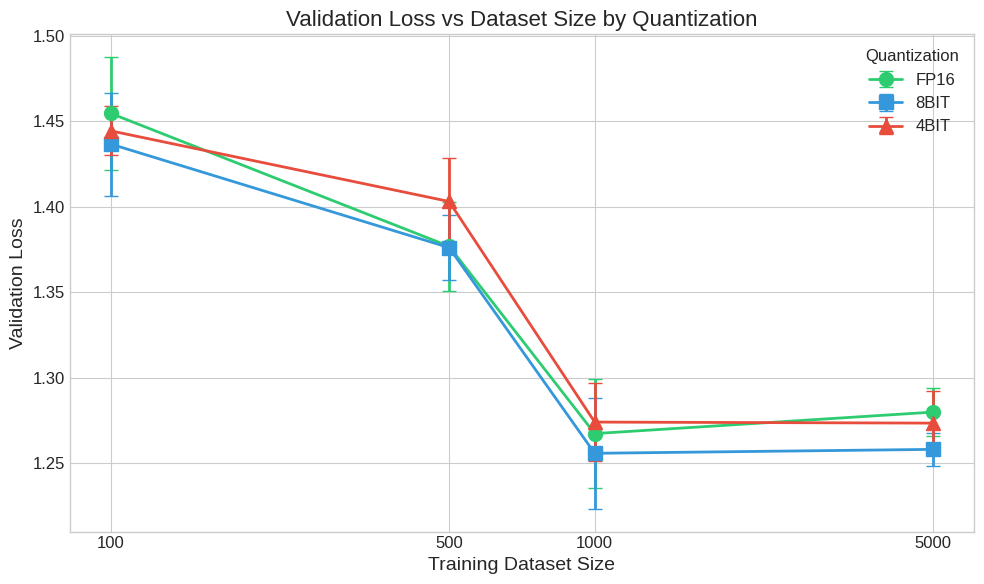
\includegraphics[width=\linewidth]{figures/figure_cell_056_00_7b.png}
    \caption{Mistral-7B: validation loss vs.\ training dataset size. 8-bit lies
      \emph{below} FP16 at every data size, with the gap widening as $n$
      increases---the opposite of H2's prediction.}
    \label{fig:val_loss_7b}
  \end{minipage}
  \hfill
  \begin{minipage}{0.48\linewidth}
    \centering
    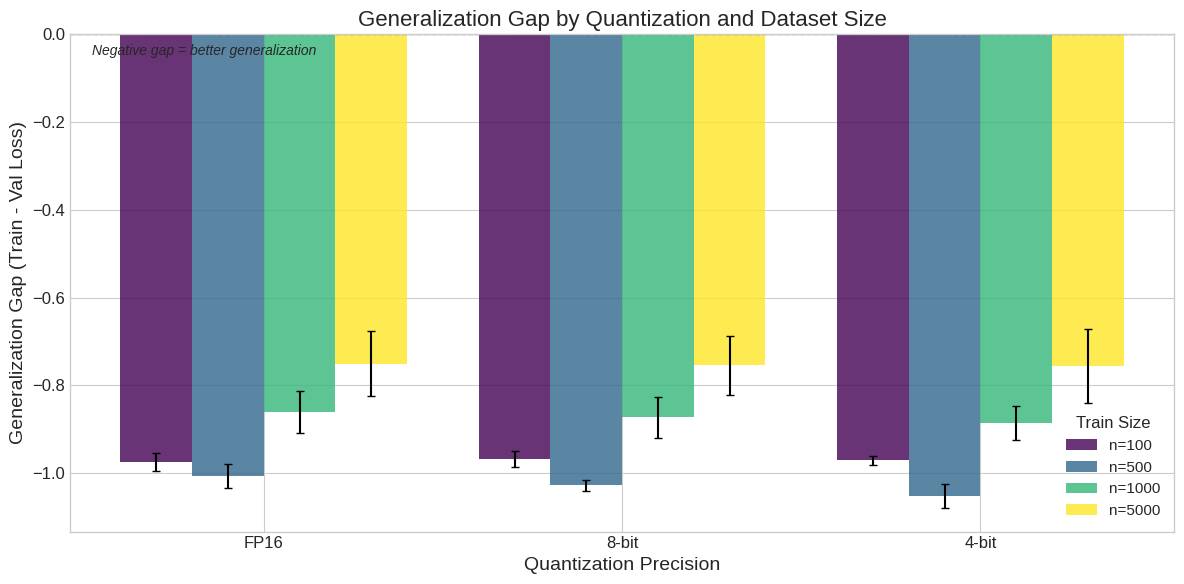
\includegraphics[width=\linewidth]{figures/figure_cell_057_00_7b.png}
    \caption{Mistral-7B: generalization gap by precision and training size.
      Unlike TinyLlama, the gaps differ more noticeably across precisions, with
      4-bit exhibiting a distinctly larger-magnitude gap than 8-bit.}
    \label{fig:gen_gap_7b}
  \end{minipage}
\end{figure}

\begin{figure}[t]
  \centering
  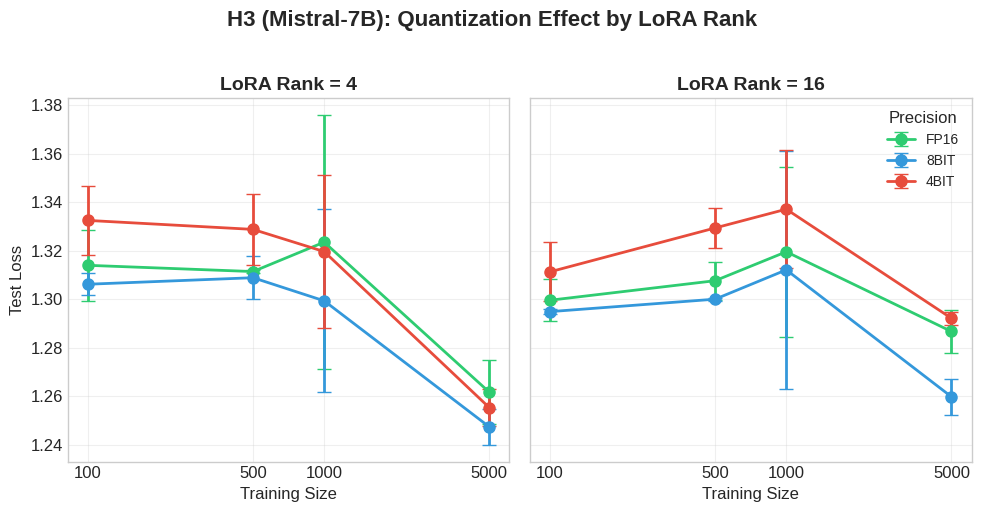
\includegraphics[width=0.88\linewidth]{figures/figure_cell_060_00_7b.png}
  \caption{Mistral-7B H3: test NLL vs.\ training size stratified by LoRA rank
    ($r \in \{4, 16\}$). At $r=4$ (left panel), 4-bit NF4 approaches and
    slightly beats FP16 at $n \geq 1000$. At $r=16$ (right panel), 4-bit
    consistently hurts. H3 is clearly supported: lower rank substantially
    reduces and can reverse the quantization penalty.}
  \label{fig:h3_7b}
\end{figure}

% -----------------------------------------------------------------------
\section{Discussion}
\label{sec:discussion}
% -----------------------------------------------------------------------

\paragraph{Why quantization does not regularize at 1.1B.}
Three mechanisms counteract the theoretical $R(\Delta)$ benefit at small scale.
\textbf{Capacity loss dominates}: quantizing a 1.1B base degrades intermediate
representations on which LoRA adapters operate, and coherent instruction-following
requires full-vocabulary fidelity that even NF4 partially destroys.
\textbf{LoRA already regularizes sufficiently}: with $r \in \{4, 16, 64\}$ on a
1.1B-parameter model, the adapter introduces at most 22M free parameters against
${\approx}51$K training tokens at $n=100$---an already favorable token-to-parameter
ratio that leaves little room for further regularization.
\textbf{Deterministic noise does not average out}: unlike stochastic regularizers
(dropout, data augmentation), quantization error $\Delta$ is a fixed,
input-independent perturbation applied identically at every step, introducing a
constant gradient bias rather than a variance-reducing perturbation.

\paragraph{Why 8-bit regularizes at 7B.}
The picture changes fundamentally at 7B for two reasons.
\textbf{Excess capacity}: a 7B FP16 model has roughly $6\times$ more parameters
than TinyLlama. Fine-tuning on 100--5000 Alpaca examples leaves a vast amount of
this capacity unutilized by the task; 8-bit's mild capacity reduction restricts
this excess without damaging core language representations.
\textbf{Loss landscape}: larger models are known to have sharper loss landscapes.
QGen's theoretical argument---that quantization noise smooths the landscape toward
flatter minima---has more to offer at 7B, where landscape sharpness is a real
constraint. The growing-with-$n$ pattern (H2 inverted) is a key signature of this
mechanism: it is precisely when optimization has run long enough to reach sharp
minima that flat-minima-inducing quantization becomes beneficial.

\paragraph{Why 4-bit still hurts at 7B (mostly).}
4-bit NF4 represents a stronger compression than 8-bit, and at low data sizes
($n \leq 500$) the representational loss in the frozen base is large enough to
outweigh the regularization benefit. Only when both data is sufficient ($n \geq 1000$)
\emph{and} rank is low ($r=4$) does 4-bit cross into beneficial territory, suggesting
a narrow operating regime where the adapter's limited capacity forces it to use the
noise-perturbed base representations constructively.

\paragraph{Practical implications.}
At $\geq\!7$B scale: 8-bit quantization should be the default choice---it saves
${\approx}50\%$ VRAM \emph{and} improves generalization by up to 0.021 NLL at
$n=5000$. 4-bit NF4 is viable when memory is the binding constraint, accepting a
moderate performance cost (0.005--0.020 NLL at low $n$; near-neutral at $n=5000$
with $r=4$). At sub-2B scale: choose quantization solely based on memory budget;
8-bit incurs $\leq 0.003$ NLL degradation; 4-bit consistently degrades by 0.012--0.019 NLL.

\paragraph{Limitations.}
The 7B scale-up uses only 2 seeds and 2 ranks, limiting statistical precision
(the large std at $n=1000$ FP16, $\pm0.036$, reflects this). We test a single
task (Alpaca instruction-tuning); structured-output or numeracy-heavy tasks may
behave differently. The per-example H4 hypothesis (quantization harms
numeracy/rare-token examples disproportionately) was not empirically evaluated.
All experiments use post-training quantization; quantization-aware training (QAT)
with learnable scales may behave differently.

% -----------------------------------------------------------------------
\section{Conclusion}
% -----------------------------------------------------------------------

We conducted a systematic empirical study of whether quantization noise in
QLoRA-style parameter-efficient fine-tuning acts as implicit regularization in
low-data instruction-tuning---and found that the answer depends critically on
model scale. At TinyLlama-1.1B, 108 controlled experiments show no regularization
benefit: FP16 consistently achieves the best or equivalent test loss, generalization
gaps are identical across precisions, and the rank-interaction is at most marginal.
At Mistral-7B-v0.1, 48 experiments reveal the opposite: 8-bit quantization
outperforms FP16 at every data size, with the benefit growing as training data
increases---a clear signature of the loss-landscape-smoothing mechanism proposed
by \citet{askarihemmat2024quantization}. The rank-interaction hypothesis is also
more strongly supported at 7B, with the 4-bit penalty being $2.2\times$ larger
at $r=16$ than at $r=4$ and even turning negative at $r=4$, $n \geq 1000$.

These findings reconcile a potential contradiction in the literature: the
QGen mechanism is real but scale-gated. At small scales, LoRA's low-rank
constraint already provides sufficient implicit regularization and capacity loss
from quantization dominates; at large scales, the model's excess representational
capacity makes 8-bit's mild compression genuinely beneficial. Practitioners fine-tuning
$\geq\!7$B models should prefer 8-bit quantization as a default; those working with
smaller models should choose precision based on memory constraints alone.

\begin{ack}
Experiments were conducted on Google Colab Pro using an NVIDIA L4 GPU (24\,GB).
We thank the developers of the Hugging Face Transformers, PEFT, bitsandbytes, and
Datasets libraries for making this work accessible.
\end{ack}

% -----------------------------------------------------------------------
% References
% -----------------------------------------------------------------------
\bibliographystyle{plainnat}
\bibliography{references}

% -----------------------------------------------------------------------
% NeurIPS Paper Checklist
% -----------------------------------------------------------------------
\newpage
\section*{NeurIPS Paper Checklist}

\begin{enumerate}

\item {\bf Claims}
\item[] Question: Do the main claims made in the abstract and introduction accurately reflect the paper's contributions and scope?
\item[] Answer: \answerYes{}
\item[] Justification: The abstract and introduction state the exact number of experiments (108 at 1.1B, 48 at 7B), report the key numerical findings (8-bit beats FP16 at 7B by up to 0.021 NLL; null result at 1.1B), and list contributions that match the experimental results in Tables~\ref{tab:main}--\ref{tab:main_7b} and Figures~\ref{fig:val_loss}--\ref{fig:h3_7b}.
\item[] Guidelines:
\begin{itemize}
    \item The answer NA means that the abstract and introduction do not include the claims made in the paper.
    \item The abstract and/or introduction should clearly state the claims made, including the contributions made in the paper and important assumptions and limitations. A No or NA answer to this question will not be perceived well by the reviewers.
    \item The claims made should match theoretical and experimental results, and reflect how much the results can be expected to generalize to other settings.
    \item It is fine to include aspirational goals as motivation as long as it is clear that these goals are not attained in the present paper.
\end{itemize}

\item {\bf Limitations}
\item[] Question: Does the paper discuss the limitations of the work?
\item[] Answer: \answerYes{}
\item[] Justification: Section~\ref{sec:discussion} explicitly discusses limitations including reduced statistical power at 7B (2 seeds), single-task scope, the unevaluated H4 per-example hypothesis, and the restriction to post-training quantization.
\item[] Guidelines:
\begin{itemize}
    \item The answer NA means that the paper has no limitation while the answer No means that the paper has limitations, but those are not discussed in the paper.
    \item The authors are encouraged to create a separate ``Limitations'' section in their paper.
    \item The paper should point out any strong assumptions and how robust the results are to violations of these assumptions (e.g., independence assumptions, noiseless settings, model well-specification, asymptotic approximations only holding locally). The authors should reflect on how these assumptions might be violated in practice and what the implications would be.
    \item The authors should reflect on the scope of the claims made, e.g., if the approach was only tested on a few datasets or with a few runs. In general, empirical results often depend on implicit assumptions, which should be articulated.
    \item The authors should reflect on the factors that influence the performance of the approach. For example, a facial recognition algorithm may perform poorly when image resolution is low or images are taken in low lighting. Or a speech-to-text system might not be used reliably to provide closed captions for online lectures because it fails to handle technical jargon.
    \item The authors should discuss the computational efficiency of the proposed approach and how it scales with dataset size, problem complexity, and so on.
    \item If applicable, the paper should discuss possible risks to privacy or fairness.
    \item While the authors might fear that complete honesty about limitations might be used by reviewers as grounds for rejection, a worse outcome might be that reviewers discover limitations that aren't acknowledged in the paper. The authors are encouraged to use their best judgment and recognize that individual actions in favor of transparency play an important role in developing norms that preserve the integrity of the community. Reviewers will be specifically instructed to not penalize honesty concerning limitations.
\end{itemize}

\item {\bf Theory Assumptions and Proofs}
\item[] Question: For each theoretical result, does the paper provide the full set of assumptions and a complete proof?
\item[] Answer: \answerNA{}
\item[] Justification: The paper is empirical. Section~\ref{sec:theory} presents a theoretical motivation adapted from \citet{askarihemmat2024quantization} without claiming new theoretical results; full proofs can be found in the cited work.
\item[] Guidelines:
\begin{itemize}
    \item The answer NA means that the paper does not include theoretical results.
    \item All the theorems, formulas, and proofs in the paper should be numbered and cross-referenced.
    \item All assumptions should be clearly stated or referenced in the statement of any theorems.
    \item The proofs can either appear in the main paper or the supplemental material, but if they appear in the supplemental material, the main paper should briefly describe what the proof shows.
    \item Theorems and Lemmas that the proof relies upon should be properly referenced.
\end{itemize}

\item {\bf Experimental Reproducibility}
\item[] Question: Does the paper fully disclose all the information needed to reproduce the main experimental results of the paper to the extent possible?
\item[] Answer: \answerYes{}
\item[] Justification: Section~4 reports all hyperparameters (learning rate, batch size, warmup, optimizer, epochs), LoRA configuration ($r$, $\alpha$, dropout, target modules), quantization parameters (threshold, dtype), dataset splits, tokenization settings, random seeds, hardware, and full library version strings for both model scales.
\item[] Guidelines:
\begin{itemize}
    \item The answer NA means that the paper does not include experiments.
    \item If the paper includes experiments, a No answer to this question will not be perceived well by the reviewers and will require justification.
    \item Reproducibility may be out of the paper's scope in exceptional cases, but if it is out of the paper's scope, the authors should still make an effort to describe what they believe the factors that influence reproducibility may be.
    \item If the code is not available, the authors should provide a high-level description of the algorithm so that a motivated reader could reproduce it.
    \item The experimental setting should be presented in the appropriate section. For example, the main assumptions underlying a theoretical result should be presented alongside the theoretical result.
\end{itemize}

\item {\bf Open access to data and code}
\item[] Question: Does the paper provide open access to the data and code used, with sufficient instructions to reproduce the main results?
\item[] Answer: \answerYes{}
\item[] Justification: The Stanford Alpaca dataset is publicly available via the Hugging Face Datasets hub (\texttt{tatsu-lab/alpaca}). Mistral-7B-v0.1 is fully open under the Apache 2.0 license (\texttt{mistralai/Mistral-7B-v0.1}). The full experimental notebook (\texttt{analysis.ipynb}) with all training, evaluation, and plotting code is included in the project repository.
\item[] Guidelines:
\begin{itemize}
    \item The answer NA means that the paper does not include experiments requiring code.
    \item Please see the NeurIPS code and data submission guidelines (\url{https://nips.cc/public/guides/CodeSubmissionPolicy}) for more details.
    \item While we encourage the release of code and data, we understand that this might not be possible in some cases, e.g., if the code contains proprietary information. In such cases, a description of the algorithm should be provided.
    \item When the paper includes a new dataset, the data collection process, and the proposed dataset should be described in detail.
    \item At submission time, the authors should make it clear which aspects of the experimental setting are already publicly available and which are novel.
\end{itemize}

\item {\bf Experimental Setting/Details}
\item[] Question: Does the paper specify all the training details (e.g., data splits, done hyperparameter search, best model selection)?
\item[] Answer: \answerYes{}
\item[] Justification: Section~4 provides complete training details for both TinyLlama-1.1B and Mistral-7B-v0.1. No hyperparameter search was performed; all hyperparameters are fixed following standard QLoRA recipes. We report results for all configurations, not just selected best runs.
\item[] Guidelines:
\begin{itemize}
    \item The answer NA means that the paper does not include experiments.
    \item The experimental details should be included in the paper or the supplemental material. If they are included in the supplemental material, the authors should provide a brief summary of the details in the main paper.
    \item The details should be accessible to the reader, regardless of whether the reader has read the supplemental material.
\end{itemize}

\item {\bf Experiment Statistical Significance}
\item[] Question: Does the paper report error bars suitably and correctly defined and does the paper report confidence intervals or statistical significance?
\item[] Answer: \answerYes{}
\item[] Justification: All reported means include $\pm 1$ standard deviation across seeds (and LoRA ranks where noted). Three seeds per configuration at 1.1B and two seeds at 7B allow assessment of run-to-run variance. Formal hypothesis tests were not conducted; we rely on the consistency of results across all 156 total runs.
\item[] Guidelines:
\begin{itemize}
    \item The answer NA means that the paper does not include experiments.
    \item The authors should answer ``Yes'' if the results are accompanied by error bars, confidence intervals, or statistical significance tests, at least for the experiments that support the main claims of the paper.
    \item The factors of variability that the error bars are capturing should be clearly stated (for example, train/test split, initialization, random seed).
    \item The method for calculating the error bars should be explained (closed form formula, call to a library function, bootstrap, etc.)
    \item The assumptions made should be validated where possible, e.g., independence, normality of the distribution of a set of runs, or
    \item The error bars should be provided for the error measure used to evaluate the main result.
    \item The exact number of runs used to compute the error bars should be stated.
\end{itemize}

\item {\bf Experiments Compute Budget}
\item[] Question: For each experiment, does the paper provide sufficient information on the computational resources (type of compute, memory, time) for reproducing experiments?
\item[] Answer: \answerYes{}
\item[] Justification: Section~4 specifies the hardware (NVIDIA L4 GPU, 24\,GB, Google Colab Pro) and total number of runs (108 at 1.1B, 48 at 7B). Per-run estimates can be derived from the reported dataset sizes and model sizes.
\item[] Guidelines:
\begin{itemize}
    \item The answer NA means that the paper does not include experiments.
    \item The paper should indicate the type of compute workers CPU, GPU or accelerator, the number of machines, and the amount of memory per worker.
    \item The paper should provide the amount of compute required for each of the individual experimental runs as well as estimate the total compute.
    \item The paper should disclose whether the full research project required more compute than the experiments reported in the paper (e.g., preliminary experiments that didn't make it into the paper).
\end{itemize}

\item {\bf Code Of Ethics}
\item[] Question: Does the research conducted in the paper conform to the Code of Ethics?
\item[] Answer: \answerYes{}
\item[] Justification: The work performs academic experiments on publicly available model weights and datasets. No human subjects are involved. The study characterizes existing methods without enabling harmful applications.
\item[] Guidelines:
\begin{itemize}
    \item The answer NA means that the paper does not require an ethics review.
    \item The authors should ensure that they comply with the Code of Ethics and describe any potential negative societal impacts of their work.
    \item If applicable, the authors should include a broader impact statement in the supplemental material.
    \item At submission time, authors do not need to fill out a consent form as this is not required until acceptance.
    \item If authors have a disability that prevents the anonymization of code or data in the submission, please contact the PC chairs for accommodations.
\end{itemize}

\item {\bf Broader Impacts}
\item[] Question: Does the paper discuss both potential positive societal impacts and potential negative societal impacts of the work?
\item[] Answer: \answerNA{}
\item[] Justification: This is an empirical study of existing fine-tuning methods on publicly available models and datasets. The work does not introduce new methods or enable novel capabilities; its primary impact is informing practitioner choices about quantization precision.
\item[] Guidelines:
\begin{itemize}
    \item The answer NA means that there is no societal impact of the work performed.
    \item If the authors answer NA or No, they should explain why their work has no societal impact or why the paper does not address societal impact.
    \item Examples of negative societal impacts include potential malicious or unintended uses (e.g., disinformation, generating fake profiles, discriminating content). The authors should also consider possible harms that could arise when the technology is used as intended, but could still cause harm in certain settings.
    \item The discussion of broader impact should be grounded in facts, careful reasoning, and speculation about reasonable scenarios. There is no need to theorize about highly speculative risks or harms.
\end{itemize}

\item {\bf Safeguards}
\item[] Question: Does the paper describe safeguards that have been put in place for responsible release of data or models?
\item[] Answer: \answerNA{}
\item[] Justification: The paper uses the publicly available Stanford Alpaca dataset, TinyLlama model weights, and Mistral-7B-v0.1 (Apache 2.0). No new models or datasets are released.
\item[] Guidelines:
\begin{itemize}
    \item The answer NA means that the paper poses no such risks.
    \item Released models that have a high risk for misuse or dual-use should be released with necessary safeguards to allow for controlled use of the model, e.g., in an anonymized fashion or requiring user authentication prior to access. Containing these risks may be in tension with the need for high quality data.
    \item If applicable, the authors should describe the dataset and model access control, and how they use data in a way that is consistent with their institutional and legal requirements.
    \item Ideally, the authors should provide an anonymized URL for evaluation purposes.
\end{itemize}

\item {\bf Licenses for existing assets}
\item[] Question: Are the creators or original owners of assets (e.g., code, data, models), used in the paper, properly credited and are the license agreements applied?
\item[] Answer: \answerYes{}
\item[] Justification: All assets are cited: Alpaca dataset~\citep{taori2023alpaca}, TinyLlama~\citep{zhang2024tinyllama}, Mistral-7B~\citep{jiang2023mistral}, bitsandbytes~\citep{dettmers2022llmint8}, PEFT/LoRA~\citep{hu2021lora}, QLoRA~\citep{dettmers2023qlora}. These are publicly released under open-source or permissive licenses (Apache 2.0, MIT, or CC-BY).
\item[] Guidelines:
\begin{itemize}
    \item The answer NA means that the paper does not use existing assets.
    \item The authors should cite the original paper that produced the code package or dataset.
    \item The authors should state which version of the asset is used if it is important for reproducibility.
    \item The number of samples used from each dataset should be provided.
    \item The text describing how assets from others were used should be in accordance with any relevant terms of service or terms of use.
\end{itemize}

\item {\bf New Assets}
\item[] Question: Are new assets introduced in the paper well documented and is the license of the new assets described?
\item[] Answer: \answerNA{}
\item[] Justification: No new datasets or models are introduced; the contribution is an empirical study using existing assets.
\item[] Guidelines:
\begin{itemize}
    \item The answer NA means that the paper does not release new assets.
    \item Newly introduced assets should be documented in detail and include a license specification.
    \item Newly introduced assets should be included in the supplemental material if possible.
    \item Crowdsourced datasets should include a detailed description of how the data was collected and processed, including instructions given to annotators and quality control measures.
    \item Authors should make sure that their dataset/code releases adhere to the terms of use of any data used when creating the dataset.
    \item Authors should consider whether the data they are releasing may be used to train models that could potentially be used in harmful ways, provide a statement on potential risks and appropriate use, and suggest safeguards where appropriate.
\end{itemize}

\item {\bf Crowdsourcing and Research with Human Subjects}
\item[] Question: Does the paper include the necessary information consistent with IRB review, or other human subjects review?
\item[] Answer: \answerNA{}
\item[] Justification: No crowdsourcing or human subjects are involved.
\item[] Guidelines:
\begin{itemize}
    \item The answer NA means that the paper does not involve crowdsourcing nor research with human subjects.
    \item Including this information in the supplemental material is fine, but if the main contribution of the paper involves human subjects, then as much information as possible should be included in the main paper.
    \item According to the NeurIPS Code of Ethics, workers involved in data collection, curation, or other labor should be paid at least the minimum wage in the country of the data collector.
\end{itemize}

\item {\bf Institutional Review Board (IRB) Approvals or Equivalent for Research with Human Subjects}
\item[] Question: Does the paper describe potential risks incurred by study participants as a result of the paper's research?
\item[] Answer: \answerNA{}
\item[] Justification: No human subjects are involved in this research.
\item[] Guidelines:
\begin{itemize}
    \item The answer NA means that the paper does not involve crowdsourcing nor research with human subjects.
    \item Depending on the country in which research is conducted, IRB approval (or an equivalent approval/review based on the requirements of your country or institution) is required for any human subjects research.
    \item If you obtained IRB approval, you should clearly state this in the paper.
    \item We recognize that the procedures for this may vary significantly between institutions and locations, and we expect authors to adhere to the guidelines that are most appropriate to their situation.
    \item Neither the authors nor their institutions should be held responsible for any violations of these guidelines occurring due to violations of these guidelines during the conduct of the research.
\end{itemize}

\end{enumerate}

\end{document}
